\svnkwsave{$RepoFile: froehlich/dailyBlog.tex $}
\svnidlong {$HeadURL$}
{$LastChangedDate$}
{$LastChangedRevision$} {$LastChangedBy$}
\svnid{$Id$}


\chapter{Research blog on symmetry reduction}
\label{chap:blog}

$\footnotemark\footnotetext{{\tt \svnkw{RepoFile}}, rev. \svnfilerev:
 last edit by \svnFullAuthor{\svnfileauthor},
 \svnfilemonth/\svnfileday/\svnfileyear}$

% J Hightower - former texas politician, author, speaker 1943-
\begin{bartlett}{
Only dead fish go with the flow}
\bauthor{
\HREF{http://www.brainyquote.com/quotes/authors/j/jim_hightower.html}
     {J Hightower}, Texas politician}
\end{bartlett}


\begin{description}
\item[2010/05/10 SF] Definition (9.9) of \emph{stabilizer}
in ChaosBook.org version13, \HREF{http://chaosbook.org/version13/chapters/discrete.pdf}
{Chapter 9 - World in a mirror} seems wrong.

\item[2010/05/10 PC] You are right - we have now
\HREF{http://www.flickr.com/photos/birdtracks/4259634492/}
{replaced ``stabilizer''} by $G_p$-\emph{symmetric} throughout the next chapter.
Please alert me to its occurrences in this chapter, suggest how to
fix them.

BTW, I referenced equation number in your remark with respect to
the stable ChaosBook.org version13 in order that it always links
 correctly: equation numbers etc. keep changing in the unstable,
 currently edited version.


\item[2010/05/11 SF]
I do not feel like I have a good grasp of Lie groups and algebras,
do you have any suggestions on what I should read to learn more
or is it not important for the research?.

\item[2010/05/12 PC]
As far as Lie groups and algebras are concerned, ignore them from now -
lets just understand what $SO(2)$ (or, equivalently $U(1)$) invariance
does to complex Lorenz equations. Physicists usually learn $\SOn{3}$ next
and not the general theory of Lie groups, so lets start small: invariance
on a circle.

\item[2010-05-13 PC] You might want to join
\HREF{http://www.zotero.org/groups/cns}
{http://www.zotero.org/groups/cns}
in order to be able to access the papers we are saving there. Nothing
urgent, for now. Search for zotero in siminos/blog/blog.pdf to find
a bit more info about it.

\item[2010/05/24] I started thinking about the problem of when the group
tangent at the point is perpendicular to the group tangent at the slice
point. I think I understand what is happening but would like you to check
my work to make sure I actually do.

    For the $x_1 = 0$ slice for the \cLe\ I think I can show that it is only possible for a trajectory to touch the slice instantaneously unless it is an {\eqv} solution: Suppose a trajectory stays in the slice for some interval of time, this means $x_1 = \dot x_1 = 0$ in this interval, which gives us that $y_1 = 0$ during this time. So $y_1$ is constant for some interval of time, so $\dot y_1=0$ here also. Looking at $\dot y_1 = 0$ when $x_1=y_1 =0$ gives $x_2 = -(e/\rho_2)y_2$. Plugging these three restrictions into the equations for $\dot x_2$ and $\dot y_2$ yield the equations $\dot y_2=-\sigma y_2 (1+(\rho_2 / e))$ and $\dot y_2 = (\rho_1 - z)(-e/\rho_2)y_2-y_2$ this means that $-\sigma y_2 (1+(\rho_2 / e))=(\rho_1 - z)(-e/\rho_2)y_2-y_2$ provided $y_2$ is nonzero, then $-\sigma (1+(\rho_2 / e))=(\rho_1-z)(-e/\rho_2)-1$. z is the only variable in that equation, so it must be constant. This means that $\dot z = -b z + x_2 y_2 + x_1 y_1=-b z+ (-e/\rho_2)y_2^2=0$. Again $y_2$ is the only variable so it too must be constant, so $x_2$ is also constant. This means the solution can stay in the slice only if all its values are constant, so it is an {\eqv} solution. There are possibly some divide by zero difficulties, but hopefully a similar argument will hold for these cases.

    So we do not run into this problem for the \cLf.

    As I understand it, the reason the group tangent along the trajectory being perpendicular to the group tangent of the slice causes problem is because this means that doing an infinitesimal rotation at the point keeps it inside the slice so the point is not a unique representative (at least when doing the infinitesimal rotations), is this correct?

    When choosing the slice to be a hyperplane through a point, it doesn't have to be perpendicular to the group tangent at some point does it? As long as the group tangent at any point isn't contained inside the hyperplane there shouldn't be a problem locally.

    I thought about trying to show that this condition being true for an interval of time implies it is always true and I have no clue how to go about it so far. I think I see why it is true if the ODE is linear like in QM, but my argument is not quite complete.


\item[2010-05-25 ES]
Linear slices are indeed not flow invariant, so only equilibria (or any
points in $\Fix{\SOn{2}}$) stay on the linear slice under equivariant
dynamics.
({\bf 2012-02-24 PC}: moved exer:SliceInvCLf to ChaosBook
exerContinuous.tex)

The trouble is that {exer:SliceInvCLf}, or what you have shown
above does not help us, I think, to conclude that the singularity at
$x_1=x_2=0$ is not reached by the dynamics. What would help, would be
exer:SingOnFixedspCLf
({\bf 2012-02-24 PC}: moved exer:SingOnFixedspCLf to ChaosBook
exerContinuous.tex)

Note that one might be even more lucky than {exer:SingOnFixedspCLf}
suggests and be able to show that we can only run into a singularity at
the origin.

\item[2010-05-28 ES] I am sure you've noticed that when you try to
integrate in invariant polynomials basis you run to some singularity - I
had never tried that before. I've only looked at your Mathematica files,
do you get the same behavior with Matlab as well? I've tried playing a
bit with the integrator, for instance using implicit Runge-Kutta should
work if stiffness and not a singularity was the problem. Any intuition on
what happens and why? If you have access to Gilmore and Letellier
book\rf{GL-Gil07b}, the section \emph{Tips for Integration} might be
helpful.

\item[2010-05-28 PC] We have the book in \wwwcb{/library}.

\item[2010-06-01 SF] I checked the differential equations for the Hilbert basis from chapter 10 of the chaos book and got a different set of a equations:
\bea
    \dot u_1 &=& 2\sigma (u_4-u_1)
        \continue
     \dot u_2 &=& 2 u_4 (\rho_1-u_5)+2 \rho_2 u_3 -2 u_2
        \continue
     \dot u_3 &=& -(\sigma+1) u_3 +\rho_2 u_1 +e u_4
        \continue
     \dot u_4 &=& \sigma u_2-(\sigma +1) u_4 + (\rho_1-u_5) u_1 - e u_3
        \continue
     \dot u_5 &=& u_4 - b u_5
\,.
\label{SF:HilbertBasEqs}
\eea

    The equations in the book are very similar to these, except $u_3$ and $u_4$ are switched, the $\rho_2$ terms are dropped (I guess since it is usually taken to be zero), and it has $\sigma-1$ instead of $\sigma+1$ in the equation for $\dot u_4$ (formerly $\dot u_3$).

    When I use this system of equations I don't have any difficulties with stiffness. I also checked the two sets of {\eqv} points for when $e+\rho_2 = 0$. They are equilibrium points for this new system, but they were not for the old. So I think this new system is the correct system, and the $\sigma-1$ was somehow causing the stiffness. I can change the formula in the book if you want, but I wanted this system to be checked before I did that.

\item[2010-06-01 ES] Stefan, thanks for catching this. The funny thing is that I had found this error in the past, corrected it in CLE paper, I copy here from \emph{revision 1449}:

==========================
    \beq
    \begin{split}
	    u_1 &= x_1^2+x_2^2 \cont
	    u_2 &= y_1^2+y_2^2 \cont
	    u_3 &= x_1 y_2-x_2 y_1\cont
	    u_4 &= x_1 y_1+x_2 y_2\cont
	    u_5 &= z\,.
	    \label{eq:ipLaser1}
    \end{split}
    \eeq

    \ES{mathematica notebook:CLEtransfJac.nb
    {\bf PC:} Changed $z$ to $u_5$; have not checked the algebra}\
    \ES{Rechecked algebra by hand, keeping $\rho_2\neq 0$. $u_3$ and $u_4$ where permuted. I will have to check
		the figures for consistency.}
\beq
\begin{split}
  \dot{u}_1 &=2\,\sigma\,(u_4-u_1)\,,\\
  \dot{u}_2 &=-2\left(\,u_2 - \rho_2\, u_3 -\,(\rho_1-u_5)\,u_4\right)\,,\\
  \dot{u}_3 &=-(\sigma\, +1)\,u_3+\rho_2\, u_1+e\, u_4\,,\\
  \dot{u}_4 &=-(\sigma\, +1)\,u_4+\,(\rho_1-u_5)\,u_1+\sigma\, u_2-e\,u_3\,,\\
  \dot{u}_5 &=u_4-b\, u_5\,.
\end{split}
\label{eq:CLEip1}
\eeq
===================================

I think it was Predrag who didn't like the formatting and copied
the Chaosbook expressions back (interchanging $u_3$ and $u_4$ one
can fit two lines in one). Anyway, my mistake, I should have immediately
corrected Chaosbook as well.

Stefan, you do use basis \refeq{eq:ipLaser1}, right?

\item[2010-06-04 SF]
I do use the basis \refeq{eq:ipLaser1} for the Hilbert polynomial
calculation.

\item[2010-06-03 PC]
Add your own text and figures. In particular,

(a) have you computed the
stability eigenvalues and eigenvectors of the \reqv\ in
the full space, Hilbert-basis reduced space and within the $x_1=0$ and
general linear slice reduced space. Evangelos has a computation in his thesis
that can probably be made shorter.

(b) would love to see how you cross the singularities when integrating
within (or rotating back into) the \reducedsp. Do a right version
of {exer:PCsectionCLe}. Discuss that in the appropriate
place in flow.tex, with your own figures. As Evangelos mentions, we
did not look at that carefully, and we do not know whether it is
possible or not to find a slice for which the strange attractor
of \cLe\ avoids the singularities altogether.
This might help you test and generalize the ideas
of your proposal of 2010/05/24 above.

({\bf 2012-02-24 PC}: moved {exer:PCsectionCLe} to ChaosBook
exerContinuous.tex)

\item[2010-06-11 SF] When I have been calculating the eigenvalues and
eigenvectors at the \reqv\ in the full space I have not been getting 0 as
an eigenvalue or the direction tangent to the group action as an
eigenvector. The eigenvalue that I thought was 0 was just really small at
the normal parameter values, but can be made larger. Also, the
determinant of the \stabmat\ at the {\reqv} isn't 0 in general.

\item[2010-06-18 SF]
I calculated the \stabmat\ for an \reqv\ when restricted to a slice by
using infinitesimal rotations and got that
\beq
{\MvarRed}(\sspRed)_{ij} = \Mvar(\sspRed)_{ij}-\velRel \cdot \Lg_{ij}
     -\groupTan(\sspRed)_i\,\left(
     \frac{\frac{\partial v}
     {\partial x_j}\cdot \sspRed}{\groupTan(\sspRed) \cdot \sliceTan{}}
     - \velRel \frac{\frac{\partial (\groupTan(\sspRed))}
              {\partial x_j}\cdot \sliceTan{}
              }{\groupTan(\sspRed)^T \cdot \sliceTan{}}
              \right)
\ee{SF:redJacob}
where $\velRel$ is the angular velocity of the \reqv, \sliceTan{} is a
vector normal to the plane, and wherever there is a `$\cdot$' it means
dot product over the symmetry group generators.
    \PC{I do not see where the sum over group symmetry generators is in
    \refeq{SF:redJacob}?}

\item[2010-07-09 SF]
I checked how close each of the approximations were to satisfying
$v(x)=J^t(\xInit) v(\xInit)$ and the Jacobian.m program, where I use the
system of differential equations, is by far the most accurate.

\item[2010-07-10 PC] I have replaced $-c I_{ij}$ in
the original Stefan's
\refeq{SF:redJacob} and \refeq{SF:redJacob1} by
$-\velRel \cdot \Lg_{ij}$, hope that is correct. Also,
I think one should first state the formula at any \statesp\
point $\ssp$, then specialize to $\ssp = \ssp_{\REQB{}}$, with
$\ssp_{\REQB{}}$ a point on an \reqv\ \REQB{} group orbit.


\item[2010-07-20 SF]
I added a matlab program, rpoNewton.m, that uses Newton's
method to find \rpo s for the \cLe. It appears to work, but
seems to be slow and you need to start close to the \rpo\ in
order for it to converge.


\item[2010-07-22 PC]
Introduced a new definition \refeq{SF:symPrimJac} of \FloquetM\ that covers
both \po s and \rpo s.

Stefan, please complete exer {traLocEigFr}~(b).

\item[2010-07-26 PC]
Stefan, I went bowling with a 12 year old on Friday, and
today I have a ridiculously bad cold, you would want to avoid
me anyway. Here is what I dreamed (not kidding!) last night
that I recommend you do:

\begin{enumerate}
    \item
Spawn off from CLE full \statesp\ plotting program a new
one that only plots a point whenever the trajectory crosses
$\groupTan(\ssp(t))^T \cdot \sliceTan{} =0$, perhaps overly these point on the chaotic
trajectory. This should give you a sense for where the
reduced states space projection is singular.
    \item
Understand where the two trajectory points immediately
bracketing above 0-crossing are in the \reducedsp,
plot only lines connecting them in the \reducedsp.
    \item
Experiment now with different choices of $(\slicep,\sliceTan{})$ to see
whether a choice can be made such that there is no
singularity on the strange attractor itself.
    \item
See whether you can select two slices, through $\slicep_1$ and $\slicep_2$
such that \reducedsp\ flow has no singularity at
all.
\end{enumerate}


\item[2010-08-16 SF]
If the hyperplane is chosen so that it does not contain the
entire invariant subspace, then it will not be possible to
rotate points `sufficiently close' to the invariant subspace
into the hyperplane (I have an idea for showing this in
general but I know its true for the \cLe ). One possible
advantage of these slices though is that the problem region
(where the group tangent is contained in the hyperplane) is
simply the boundary between the points that can be rotated
into the plane and the points that cannot be (again I have an
idea for how to show this in the general case but I only know
it for a fact with the S0(2) symmetry).

When we reach the problem area for one of these hyperplanes,
we could just move to another one that covers this new region
'closer' to the invariant subspace. If we only care about a
region that doesn't get infinitely close to the invariant
subspace then we can use a single hyperplane, but if it does
go infinitely close the invariant subspace then we would need
infinitely many of these planes.

I don't know a general description for the problem region
when the slice does contain the entire invariant subspace,
but these hyperplanes seem to be able to have any point
rotated into them. For these hyperplanes the entire group
orbit of the problem points is contained in the problem
region, whereas in the other case only a finite number of
points on the group orbit have the group tangent in the
direction of the plane.

\item[2010-08-16 PC]
I agree that if you take a slice \emph{not} orthogonal to the group
tangent $\sliceTan{}$ at the slice-fixing point $\slicep$,
so that the group {\fixedsp}, \ie,
$\pS_H$ of a subgroup or a `centralizer' $H \subset \Group$
\refeq{dscr:FPsubsp} is not included, the slice is no
good. An example for \cLe\ would be a slice
that does not include the $z$-axis.
But are you sure that for our orthogonal definition
of slice there are parts of {\statesp} with larger symmetry
that stick out of the slice? Waiting for an example...
\index{centralizer}\index{fixed-point subspace}
\index{G-fixed@\Group-fixed}\index{fixed point!under \Group}

\item[2010-08-17 SF]
Oh, I meant that in general it was possible to have slices that couldn't be rotated into. If the slice is chosen orthogonal to the direction of symmetry then it should always contain the fixed-point subgroup since: if $\pS_H$ is the fixed point subgroup and $x \in \pS_H$ then $T_a x=0$ since $x$ is unchanged by the group elements and if $y$ is any point then $x \cdot T_a y=T_a^* x \cdot y=-T_a x \cdot y=0$ (where $T_a^*$ is the Hermitian conjugate)

Does the slice need to have the fixed-point subgroup in order to be useful? We should be able to chose slices arbitrarily close to containing the fixed-point subgroup, or will that still not be enough?

\item[2010-08-18 SF]
Here are a couple of 'idea/proofs' that using a slice orthogonal to a group tangent will always be able to have the entire space rotated into it. I'm not entirely sure if they are valid though
\begin{enumerate}
    \item
We want to show that when we fix $x$ and let $y$ be any point in the {\statesp}, there exists $\theta_a$ such that $<T_a x|e^{T\cdot \theta}y>=0$, (where $T \cdot \theta=\sum T_a \theta_a$) for every $T_a$.
To do this consider the function $f_y(\theta)=<x|e^{T \cdot \theta} y>$. Provided all its partial derivatives exist and it has a minimum, then the minimum must have all the partial derivatives equal to 0. $\frac{\partial f_y}{\partial \theta_a}=<x|T_a e^{T \cdot \theta} y>=<T_a^* x|e^{T \cdot \theta} y>=<-T_a x|e^{T \cdot \theta} y>$ so the minimum must be a point where $-<T_a x|e^{T \cdot \theta} y>=0$. This means that the minimum (or any extrema) of $f_y$ is a point on the orbit of $y$ in the slice.
In order for this proof to be valid we need (i) that $f_y$ is differentiable and (ii) $f_y$ has a minimum (or any extrema). (i) seems like it follows from the fact that $e^{T \cdot \theta}$ is differentiable and (ii) should follow if the group orbits are compact (is this true in general for a compact Lie group?) and if $f_y$ is differentiable then it is continuous, so it must be bounded on any group orbit.
    \item
The next idea was motivated by observations from SO(2) that I do not know if they hold in general.

The second idea is to look at the functions $f_a(y)=<\groupTan(x)_a| y>$. $ y$ is in the slice normal to the group actions at $x$ if $f_a(y)=0$ for every $a$. From my comment yesterday, we already know that any point in the fixed-point subspace is a zero of the function. I don't know enough about compact Lie groups to say whether or not this is possible, but construct a region R with the properties (i) It is contained in a hyperplane, L, in the {\statesp}, (ii) the group orbit of the point we are looking at is the boundary of R in L, (iii) a point of the fixed-point subspace is contained in the interior of R in L. For SO(2), these are just the circles that the rotations around the z-axis form the boundary of. Once we have this region R, then we know that $f_a$ has a zero inside of R (the point from the fixed-point subspace) and $f_a$ is linear. From the point in the fixed-point subspace, go in a direction normal to the gradient of $f_a$ until it reaches the boundary. $f_a$ is linear so this direction is always normal to the gradient so the value of $f_a$ was not changed by this. That means this point is a zero of $f_a$. If we choose a direction normal to the gradient $f_a$ for every a, then we find a point that is a zero for all of the $f_a$ and on the boundary of R in L, meaning we found a point in the group orbit that is in the slice.
\end{enumerate}

\item[2010-08-20 SF: Linear \slice s]
For \mslices\ to be operationally useful, we first must show that a \slice\ \refeq{PCsectQ1}
cuts the group orbit of every point in the full \statesp.

Let $\ssp \in \pS$ be a point in the \statesp, and $\Group$ be Lie group with group elements represented  by $\LieEl=e^{\gSpace \cdot \Lg}$, as in \refeq{FiniteRot}.
    \PC{this looks like a repeat of what is to come, dropped: `` We want to show that there is a point on the group orbit of $\ssp$ which lies in \pSRed, \ie\ there exists a group element $\LieEl=e^{\gSpace \cdot \Lg}$, $\sspRed= \LieEl \ssp \in \pSRed$ such that $\braket{\LieEl \ssp}{\sliceTan{a}}=0$ for all $a$.
    ''}

Consider $f(\gSpace)=\braket{e^{\gSpace \cdot \Lg} \ssp}{\slicep}$, the projection of the group orbit of $\ssp$ onto the slice-fixing ray through \slicep\ (If the {\statesp} is real, this differs by a constant from $\|e^{\gSpace \cdot \Lg}\ssp - \slicep\|$, the function used in\rf{rowley_reconstruction_2000,rowley_reduction_2003} to find a point in a slice).
$f$ is a continuous and differentiable function of \gSpace. If $\ssp$ is the invariant subspace \refeq{def:centralizer}, its group orbit is itself and $f(\gSpace)$ takes a constant value.

If $\gSpace_E$ is an extremum of $f$ then all of the first order partial derivatives of $f$ vanish at $\gSpace_E$, $\frac{\partial f(\gSpace_E)}{\partial \gSpace_a} =\braket{\Lg_a e^{\gSpace_E \cdot \Lg} \ssp}{\slicep}=0$. $\Lg_a$ is antihermitian, so
$0=\braket{\Lg_a e^{\gSpace_E \cdot \Lg}\ssp}{\slicep}
= - \braket{\LieEl_E \ssp}{\Lg_a  \slicep}$,
and
\[
\braket{\LieEl_E \ssp}{\sliceTan{a}} =0
\,.
\]
We therefore have that $\sspRed= \LieEl_E \ssp$ is normal to all the group tangents of $\ssp$ so it is in \pSRed. This means that the slice condition is satisfied by $\sspRed_E = \LieEl_E \ssp$ corresponding to an extremum of $f$, and thus $\sspRed_E$ is in the slice (for $\mathbb{R}^n$ this is equivalent to looking for the extrema of $\|e^{\gSpace \cdot \Lg}\ssp - \slicep\|$\rf{rowley_reconstruction_2000,rowley_reduction_2003}, so this says that any points that are locally the closest or the farthest from a our slice fixing point will be in the slice). All that is left to do then is to show that $f$ has extrema. But as the group is compact, the group orbit of every point in \pS\ is compact, so its projection on the slice-point $\slicep$ has at least two extremal points, and thus every group orbit intersects the \slice. For example, group orbits of \SOn{2}\ are topologically circles, and their projections have maxima, minima and inflection points as extrema.
    \PC{drop this text eventually}
    \PC{
    Stefan, if I have removed some essential part of your proof, please restore it.
    The narrative continues in \refsect{sect:sliceSing}.
    }



\item[2010-08-31 SF]
Some things that I have been looking at:

\begin{enumerate}
\item
I think the first 'proof' I gave that any element can be rotated into a hyperplane defined by being normal to the group tangents at a point actually works (provided the Lie group is connected so that we can use the $e^{T \cdot \theta}$ representation for any group element): The only thing that remained to be shown was that the function had extrema. To show this, instead of looking at $f_y(\theta)=<x|e^{T \cdot \theta} y>$ consider the function $g_x(z)=<x|z>$ on the group orbit of $y$. The group orbit of y is compact in the {\statesp} since we are looking at a compact Lie group and $g_y$ is just a linear function so it is continuous. So we are looking at a continuous function on a compact space, so the function obtains both its maximum and minimum. Let $z_{min}$ be the point where the function achieves its minimum. $z_{min}$ is in the group orbit of $y$ so there is a $\theta_{min}$ such that $z_{min}=e^{T \cdot \theta_{min}}$. Now notice that since we restricted the function to group orbit of y, for any $\theta$ there is a point $z(\theta)$ such that $e^{\theta \cdot T}=z(\theta)$. This means that $f_y(\theta)=g_x(z(\theta))$ so $\theta_{min}$ must be a minimum of $f_y$ since $x_{min}$ is a minimum of $g_x$.

\item
I looked at what happens when we map lines into a slice with a group tangent as a normal vector. Every time I did this with a line that passed through a point in the slice where the group tangent is normal to the slice point, I found that the $\theta$ used to rotate the line into the slice was the same for the entire line, meaning that $\dot \theta$ is zero everywhere along the line in the reduced space and that it is just a removable discontinuity. I haven't thought about how to show whether this is true in general yet.

\item
I also looked at a some trajectories that in reduced space looked like they might have jumps that meant they passed close to a singularity, but whenever I looked at the trajectory along these 'jumps', I found that the trajectory was actually smooth along these and that the dot product of the group tangent at the point and the normal vector to slice were far from zero at these points. I used initial points that were in the strange attractor. None of these trajectories actually passed through a singularity as far as I know. Tomorrow I will look at trajectories passing near to a singularity to see how they look at these points.

\end{enumerate}

I have mathematica programs for the last two things, but I don't have enough time before my next class to comment them so that they would make sense, but I will add them/show them to you tomorrow.

\item[2010-09-17 SF]
For $\SOn{2} \times \SOn{2}$, where each group acts on the invariant subspace of the other, it appears that only one of the second order partials has to be 0 in order for there to be a problem.

Let $\Lg_1$ and $\Lg_2$ be the infinitesimal generators for the two $\SOn{2}$ groups. We have chosen the group so that $\Lg_1 \Lg_2=0$.
    \PC{$\Lg_1$ and $\Lg_2$ commute, $[\Lg_1, \Lg_2]=0$. But their product is definitely not zero, that would mean that one could not walk straight and sidewise at the same time - only President Ford could not do that. Anyway, I think what shows up in infinitesimal transformations are the sums, not the products of generators.}
We know that for any $\gSpace$ used to rotate the trajectory,
\beq
\velRed(\sspRed) = \vel(\sspRed)-\dot{\gSpace}(\sspRed) \cdot \groupTan(\sspRed)
\eeq
so when we restrict it to a \slice\ normal to $\groupTan_1(\ssp')$ we get that

$<\vel(\sspRed)-\dot{\gSpace}(\sspRed) \cdot \groupTan(\sspRed)|\groupTan_1(\ssp')>=$

$<\vel(\sspRed)|\groupTan_1(\ssp')>-<\dot{\gSpace_1} \groupTan_1(\sspRed)|\groupTan_1(\ssp')>-<\dot{\gSpace_2} \groupTan_2(\sspRed)|\groupTan_1(\ssp')>=0$.

We know that
$<\dot{\gSpace_2} \groupTan_2(\sspRed)|\groupTan_1(\ssp')>=0$ since $\Lg_1 \Lg_2=0$.
This leaves us with $<\vel(\sspRed)|\groupTan_1(\ssp')>-\dot{\gSpace_1}<\groupTan_1(\sspRed)|\groupTan_1(\ssp')>=0$ which gives us the equation for $\dot{\gSpace_1}$:
\beq
\dot{\gSpace_1}=\frac{<\vel(\sspRed)|\groupTan_1(\ssp')>}{<\groupTan_1(\sspRed)|\groupTan_1(\ssp')>}
\eeq
There is only $\Lg_1$ in the denominator, so the projection on the first group tangent is the only one that has to have the second partial equal to zero in order for the point to have a singularity.

I guess this makes sense since if a point $\sspRed$ is in the slice normal to $\groupTan_2(\ssp')$ then any point in the $\Lg_1$ orbit is in the slice since $<e^{\gSpace_1 \Lg_1}\sspRed|\groupTan_2(\ssp')>=<(1+\gSpace_1 \Lg_1+\ldots)\sspRed|\groupTan_2(\ssp')>=<\sspRed|\groupTan_2(\ssp')>+<\gSpace_1 \Lg_1 \sspRed|\groupTan_2(\ssp')>+\ldots=0$. The first inner product is zero because we assumed that $\sspRed$ was in the slice and the rest of terms are zero because $\Lg_1 \Lg_2=0$. So the only restriction for the values of $\gSpace_1$ that rotate the point into the slice are the restrictions it gets from the $\groupTan_1(\ssp')$ condition.

The condition that all second partial derivatives are 0 seems to be a stronger condition than what we are looking for.

One other thing that I'm not sure if its useful/important:

I looked into what the conditions were for there to be a continuous trajectory in the intersection of the slice and group orbit; \ie\ given a slice fixing point $\ssp'$ and any point $\sspRed$ in the slice, what are the conditions so that there is a differentiable trajectory $\gSpace(s)$, $s\in(0,1)$, with $<e^{\gSpace(s)\cdot \Lg}\sspRed|\groupTan_a(\ssp')>=0$ for each $a$ and $s\in(0,1)$. For this to be true, the derivative of this equation must be zero for all $s\in(0,1)$.
When you do this you get that $\dot{\gSpace}$ must satisfy $M_{ij}\dot{\gSpace_j}=0$ where $M_{ij}=<\groupTan_j(\sspRed)|\groupTan_i(\ssp')>$. This matrix is symmetric since the commutators $[\Lg_i,\Lg_j]$ are linear combinations of the $\Lg_k$ (I believe you showed this in your book), $M_{ij}=<\groupTan_j(\sspRed)|\groupTan_i(\ssp')>=-<\sspRed|\Lg_j \Lg_i \ssp'>=-<\sspRed|([\Lg_j,\Lg_i]+\Lg_i \Lg_j)\ssp'>=-<\sspRed|[\Lg_j,\Lg_i]\ssp'>-<\sspRed|\Lg_i \Lg_j \ssp'>=-<\sspRed|[\Lg_j,\Lg_i]\ssp'>+<\groupTan_i(\sspRed)| \groupTan_j(\ssp')>=0+M_{ji}$ ($<\sspRed|[\Lg_j,\Lg_i]\ssp'>=0$ since $[\Lg_j,\Lg_i]=C_{ijk}\Lg_k$ for some $C_{ijk}$ so $<\sspRed|[\Lg_j,\Lg_i]\ssp'>=C_{ijk}<\sspRed|\groupTan_k(\ssp')>=0$ since $\sspRed$ is in the slice).
So if we can get an understanding of the null space of this symmetric matrix, then we can determine if there will be a singularity.

It also shows up if you look at the equation for the \reducedsp\ trajectory like what was done earlier, you get that for $\dot{\gSpace}$ to rotate the trajectory into the slice, it must satisfy $V_i-M_{ij}\dot{\gSpace_j}=0$ where $V_i=<\vel(\sspRed)|\groupTan_i(\ssp')>$ and $M$ is the matrix from before.

All the second partial derivatives vanishing for the projection on to the slice fixing point corresponds to when this matrix is 0. So it seems that the entire group orbit is in the slice when all the second partials are zero.

When I looked at this matrix for $\SOn{3}$, its null space always has dimension at least one at any point, but I don't know if these directions can be made into a trajectory that satisfies the condition.

\item[2010-09-21 SF]
The first result for when $\Lg_1 \Lg_2=0$ is in the previous entry.
For when we look at different representations for $\SOn{2}$: we have that $\velRed(\sspRed) = \vel(\sspRed)-\dot{\gSpace}(\sspRed) \cdot \groupTan(\sspRed)$, so for the velocity to stay in the slice we must have $<\velRed(\sspRed)|\groupTan(\ssp')>=<\vel(\sspRed)-\dot{\gSpace}(\sspRed) \cdot \groupTan(\sspRed)|\groupTan(\ssp')>=0$ so $<\vel(\sspRed)|\groupTan(\ssp')>-\dot{\gSpace}(\sspRed)<\groupTan(\sspRed)|\groupTan(\ssp')>=
<\vel(\sspRed)|\groupTan(\ssp')>+\dot{\gSpace}(\sspRed)<\sspRed|\dual{\Lg} \Lg \ssp'>=0$ giving us
$\dot{\gSpace}(\sspRed)=-\frac{<\vel(\sspRed)|\groupTan(\ssp')>}{<\sspRed|\dual{\Lg} \Lg \ssp'>}=-\frac{<\vel(\sspRed)|\groupTan(\ssp')>}{<\sspRed|\sum_\alpha C_2^{(\alpha)} \, \id^{(\alpha)} \ssp'>}$

The sum over the irreducible spaces is still in the denominator

\item[2010-10-12 SF: Submitted GT competition paper]
``Reducing continuous symmetries with linear slice,''
to Georgia Tech SAIC Student Paper Competition\rf{Froeh10}.
The paper is embedded into this blog.tex,
contained within the
\begin{verbatim}
	\ifarticle ... \else ... \fi
\end{verbatim}
article switches.


\item[2010-10-20 SF: Template fitting] In
    \refref{rowley_reconstruction_2000}, the authors use a technique
    called template fitting to reduce the dynamics of translationally
    equivariant systems.

The strategy behind template fitting is to shift the data so that at
any time it matches as closely as possible with a preselected
template function. Let $f:\mathbb{R}\rightarrow\mathbb{R}$ be a
$2\pi$ periodic function that we are fitting to a $2\pi$ periodic
template function $f_0$. The goal is then to find the value of $c$
that minimizes the square of the norm of the difference of the two
functions: \bea &&\int_0^{2\pi} [f(\ssp-c)-f_0(\ssp)]^2 d\ssp
\continue &=& \int_0^{2\pi} [f(\ssp)-f_0(\ssp+c)]^2 d\ssp \continue
&=& \int_0^{2\pi} f^2(\ssp)-2 f(\ssp) f_0(\ssp+c)+f_0^2(\ssp+c) d\ssp
\continue &=& \int_0^{2\pi} f^2(\ssp)
d\ssp+\int_0^{2\pi}f_0^2(\ssp+c)d\ssp-\int_0^{2\pi}
f(\ssp)f_0(\ssp+c)d\ssp \continue &=& \int_0^{2\pi} f^2(\ssp)
d\ssp+\int_0^{2\pi}f_0^2(\ssp)d\ssp-\int_0^{2\pi}
f(\ssp)f_0(\ssp+c)d\ssp \eea where we use the fact that both
functions have period $2\pi$ to shift the intregrals by $c$. The
first two integrals are independent of the choice of $c$, so finding
this minimum is the same minimizing $-\int_0^{2\pi}
f(\ssp)f_0(\ssp+c)d\ssp$. This is the same as maximizing
$\braket{f(\ssp)}{f_0(\ssp+c)}$, where the inner product is the
standard inner product on $L^2[0,2\pi]$ \refeq{innerL2}.

If $c$ maximizes $\braket{f(\ssp)}{f_0(\ssp+c)}$, then assuming
differentiability it must be a critical point \beq
\partial_c \braket{f(\ssp)}{f_0(\ssp+c)}=0
\eeq which is equivalent to $\braket{f(\ssp)}{f_0'(\ssp+c)}=0$.
Shifting the integral by $c$ we get the condition \beq
\braket{f(\ssp-c)}{f'_0(\ssp)}=0. \eeq

Suppose we are working with a translational equivariant dynamical
system. Let $\LieEl_c$ be the group element that corresponds to
translating by $c$. Let $u(\ssp,\tau)$ be a solution to the system.
When we fit $u(\ssp,\tau)$ to the template $u_0(\ssp)$ we are finding
$c(\tau)$ such that $\braket{\bar{u}}{u'_0}=0$, where
$\bar{u}(\ssp,\tau)=u(\ssp-c(\tau),\tau)=\LieEl_{c(\tau)}u(\ssp,\tau)$.
We are finding an equivalent trajectory to $u$ that is normal to
$u_0'$.

Consider an infinitesimal translation by $\delta c$. $u_0(\ssp+\delta
c,\tau)=u_0(\ssp,\tau)+\delta c \, u'_0(\ssp,\tau)$, so from
\refeq{eq:infinitesimal} we know that the group tangent at $u_0$ is
$u'_0$.

This means that template fitting is simply translating the trajectory
to get a reduced trajectory normal to the group tangent of the
template function. This is the same as taking a linear slice
\refeq{def:slice} with slice fixing point $u_0$. The reduced
trajectory is found by maximizing $\braket{f(\ssp)}{f_0(\ssp+c)}$,
which is the function used in 2010-08-20 post.

\bigskip
[PC moved these to blog from the SAIC paper\rf{Froeh10}:]
 We formalize these observations by following definitions:

\begin{definition}
\textbf{\Slice.} If $\Group$ acts `regularly' on a d-dimensional
manifold $\pS$, \ie\ all its group orbits are $N$ dimensional, then
we define a
\emph{slice}\rf{CartanMF,FelsOlver98,FelsOlver99,OlverInv} through a
point $\slicep$ to be a $(d\!-\!N)$ dimensional submanifold $\pSRed$
such that all group orbits in an open neighborhood of $\slicep$
intersect $\pSRed$ transversally and only once.
\end{definition}

\begin{definition}
\label{def:slice}
\index{slice}
\textbf{Linear \slice.}
Pick a non-zero \emph{slice-fixing point} $\slicep \in \pS$.
We call the $(d\!-\!N)$-dimensional hyperplane $\sspRed \in \pSRed$
a \emph{linear \slice}, where
\(
\braket{\sspRed - \slicep}{\sliceTan{a}}=0
\) %ee{PCsectQ1}
is normal to all group tangents $ \sliceTan{a}= \Lg_a \slicep$ at $\slicep$. The {slice-fixing point} should lie outside the invariant subspace $\pS_\Group$ or any of the invariant subspaces $\pS_H$ defined in \refeq{dscr:FPsubsp}. Were \slicep\ invariant under the group, then $\sliceTan{a}=0$ and the `\slice' so defined would be the entire space.
    \PC{Extend this claim to the invariant subspaces as well}
    \PC{In constructing his return map, Lorenz, I think,
    used projections on the invariant axes $z$ and $\dot{z}$.
    Is that not a \slice? Rethink}

As $ \braket{\slicep}{\sliceTan{a}}=\braket{\slicep}{\Lg_a \slicep} =0 $
by the antihermiticity of \Lg, the condition that a point \sspRed\ lies
in the \slice\ \pSRed\ reduces to
\beq
\braket{\sspRed}{\sliceTan{a}}=0
    \,,\qquad
\sliceTan{a} = \Lg_a \slicep
\,.
\ee{PCsectQ1}
\end{definition}


\begin{definition}
\label{def:movingFrame}
\index{moving frame}
\textbf{Moving frame.}
For any $\ssp$, the slice condition \refeq{PCsectQ1} on $\sspRed =
\LieEl(\gSpace)\ssp$ determines the group
action $\LieEl(\gSpace)$ that brings $ \ssp$ into the \slice.
We begin to fix the unique \reducedsp\ by requiring that the crossing is
oriented:
\beq
\braket{\groupTan_{}(\ssp)}{\sliceTan{}} > 0.
\ee{SF:orientedSlice}
In general this will not be sufficient to select unique representative and additional constraints are required.
If there is a set of angles
$\{\gSpace_1\leq\gSpace_2\leq\cdots\leq\gSpace_k \}$ that
satisfy the oriented slice transversal conditions
\refeq{PCsectQ1}, \refeq{SF:orientedSlice}, we take the
smallest angle $\gSpace_1$.
    \PC{problem: this makes sense only for \SOn{2}}
Such a map from a point in the full \statesp\ to the group action
$\gSpace$ is called a
\emph{moving frame}\rf{FelsOlver98,FelsOlver99,OlverInv}.
\end{definition}

While in general a {\slice} need not be a hyperplane,
we find the linear slice condition \refeq{PCsectQ1} easiest to implement.
For the linear case, the same slice is fixed by any
point on the ray $const\; \slicep$ through the point \slicep.
In this paper, whenever we use the term \slice\ it will refer to a
hyperplane as in the above definition. The main focus of this paper is
these linear slices.

\item[2010-11-13 PC: Linear algebra]
I like discussion of norms and least square problems \etc\
in Trefethen and Bau\rf{Trefethen97}.

\item[2010-11-20 PC: Norms]
I like discussion of norms in Stone and Goldbart\rf{StGo09}.

\item[2010-11-18 PC:]
Stefan Froelich won one of the six awards in the Georgia Tech 21st Annual
SAIC Student Paper Competition. There were 2 undergraduate finalists and
10 graduate finalists.

\item[2010-11-19 PC: Figure formatting secrets]
Tried to find some sample fig*.m code for Stefan, added
froehlich/mathematica/Fig\_CmplxContour.m , but if Evangelos has
documented his figures somewhere, he'll take that secret to his grave.

\item[2010-11-19 SE:]
The truth is that after a few years of working without realizing I
should document the figures, I did the dumbest thing I could and
decided to document them as comments in the figures of papers, blogs,
etc..
Anyway, I did not use any .m files for producing figures, I always did
it interactively through the notebooks.

\item[2010-11-20 PC:] I think that is very good - if one likes a figure
in a publication, one can go search for the code that produced it, and
having it noted in the raw manuscript is the most effective way.

Annotating them in a single list in figSrc/00ReadMe.txt file is the way I
find it easiest to track them, but it might be too much work...

\item[2010-11-19 SE:]
The problem I have with this approach is that many figures do not make
it to the final version of the paper and then I have no documentation
on how I produced them. 00ReadMe.txt is the way to go...

vaggelis/testing/flows/CLEfinal.nb

might give you an idea of what I use for plotting. It's usually very
complicated though, because I have to plot everything 3 times so that
I get reasonable size figures. I could perhaps work directly on
Stefan's notebook?

\item[2010-11-20 RLD:]
If Stefan is not able to get it done with Mathematica, then I do have all
the Matlab scripts (so called m-files) for figures I produced for out
paper, as well as my other papers.  I'll be happy to share them. if
Stefan wants to look through the figures in our KS paper and choose the
ones that are similar to what he wants to do, I can send him m-files for
them.

\item[2010-12-20 Stefan, 2011-01-13 Predrag]
Slice \&\ dice article figures drawn. [2011-01-13] The white borders have
been trimmed, so figure fills the entire frame in both height and width.

 \begin{figure}
 (a) 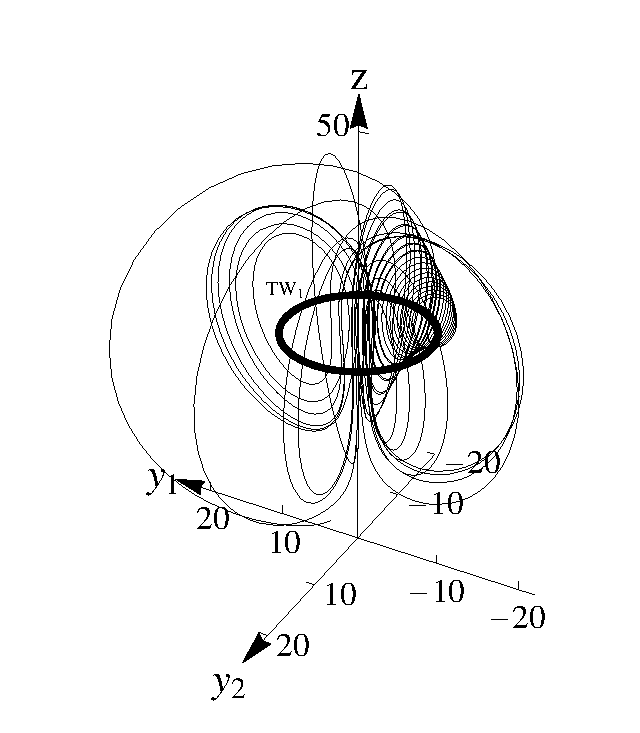
\includegraphics[width=0.35\textwidth]{Fullspace}%
 (b) 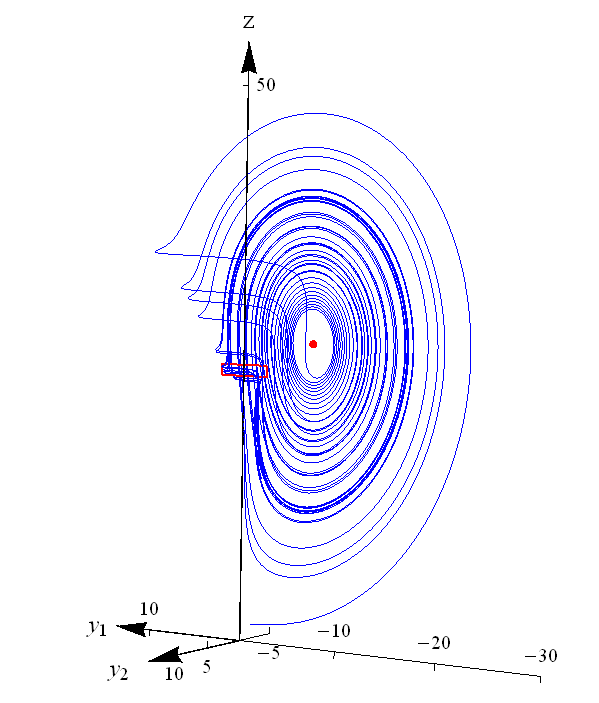
\includegraphics[width=0.35\textwidth]{RedTrajNoPlane1}%
 (c) 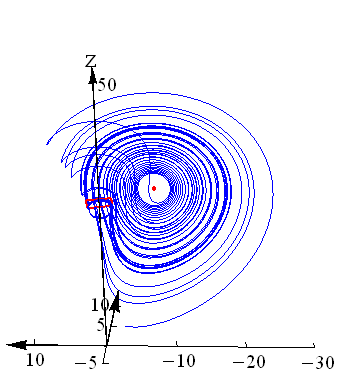
\includegraphics[width=0.35\textwidth]{RedTrajNoPlane2}%
 \caption{\label{fig:Fullspace}
(a), (b) Look good, transferred to `slice.'
(c) Probably the best, as it shows the semicircle that you then
blow up in \reffig{fig:singpass}.
 }%
 \end{figure}

 \begin{figure}
 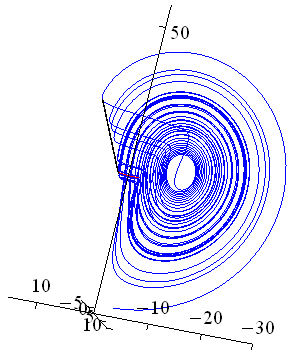
\includegraphics[width=0.35\textwidth]{RedTrajPlane1}%
 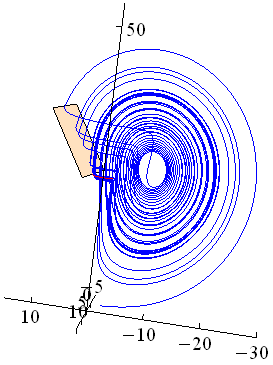
\includegraphics[width=0.35\textwidth]{RedTrajPlane2}%
 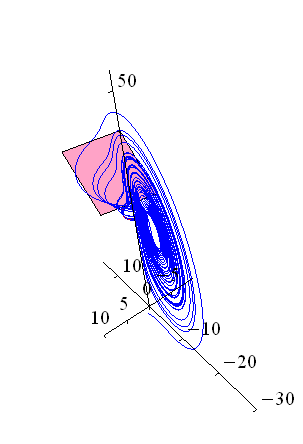
\includegraphics[width=0.35\textwidth]{RedTrajPlane3}%
 \caption{\label{fig:RedTrajPlane1}
Not sure we can draw a plane that illustrates the
3$d$ singularity space.
Stefan, write the caption.
 }%
 \end{figure}

 \begin{figure}
 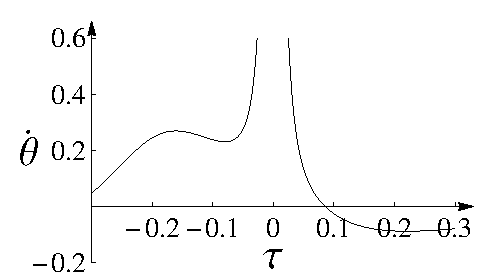
\includegraphics[width=0.40\textwidth]{dthetanearsing}%
 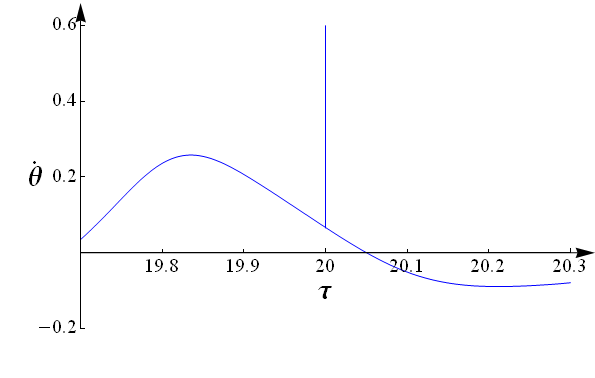
\includegraphics[width=0.40\textwidth]{dthetasing}%
 \caption{\label{fig:dthetanearsing}
Looks good, transferred to `slice.'
 }%
 \end{figure}

 \begin{figure}
 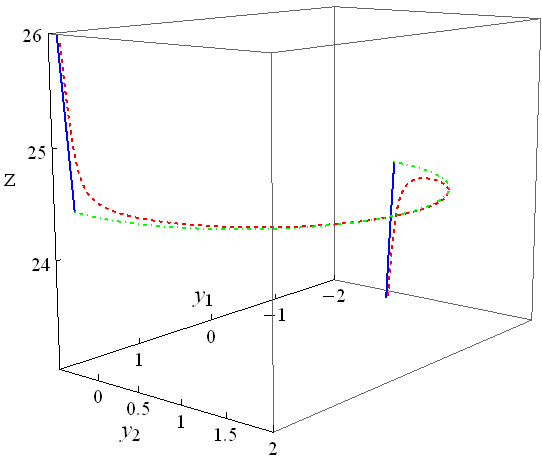
\includegraphics[width=0.35\textwidth]{singpass1}%
 \caption{\label{fig:singpass1}
Looks good, transferred to `slice.'
 }%
 \end{figure}

\item[2010-12-21 PC to Stefan] Not sure how much I'll be able to do while
in Zagreb, and I do not have time today to critically pick out the
figures that would be the best suited. My suggestion is that you enter
here captions for the figures and whatever text you write for the body of
the article, and I merge them once I am back Dec 28.

\item[2011-01-12 PC to Stefan]
In slice paper figures
%\reffig{fig:dthetasing}\,(b) and \reffig{fig:singpass}\,(a)
you use a full \statesp\ perturbation $\delta \ssp$. Would it be more consistent
to perturb with $\delta \sspRed$?

\item[2011-01-13 SF]
I used the perturbation $\delta \ssp$ because I was calculating
    the trajectories in the full space and then reducing them.
    dy=(-0.0246486, 0.00417712, 0., 0., 0.) if you want to use it.

\item[2011-01-13 PC to Stefan]
full \statesp\ perturbation $\delta \ssp$ is good enough, we stick to it.

\item[2011-01-24 ES] Critique of Figure 2 in Froelich and Cvitanovi\'c: As our
reviewer of CLE paper suggested, using $g(\tau)$ is not really transparent and
needs some explanation..

\item[2011-01-24 PC]
You are right. Now I wrote ``
Any \statesp\ trajectory can be written in a factorized
form $\ssp(\tau)=\LieEl(\tau)\,\sspRed(\tau)$
(here $\LieEl(\tau)$ is a shorthand for $\LieEl(\gSpace(\tau))$,
or perhaps even $\LieEl(\gSpace(\ssp(\tau)))$).
''

\item[2011-01-24 ES]
In the caption for part (b) you mention 3 hyperplanes:
the slice, the ``hyperplane of inflection points'' and finally their intersection
which you call inflection hyperplane $S$. It's like saying there is more
inflection associated with $S$ than with the
``hyperplane of inflection points.'' And in any case the two names are too
similar to be used in the same context. This is what confused me in the text
discussing the same issue.
I would suggest sticking with ``singular set'' for $S$. A related point is that
you might want to avoid speaking about inflection in the abstract or introduce
it properly. As it stands I think it is not clear what it refers to.

\item[2011-01-24 PC] You are right, I now tried to get rid of the first
``hyperplane of inflection points''. ``Inflection hyperplane'' is a
macro, can be reverted to ``singular set'' at a whim. I went away from it
to emphasize that it is \emph{a hyperplane} (it's surprising that these
lie in a hyperplane, ``set'' is for wimps, just a bunch of points), and
\emph{inflection} hyperplane, because zillion things are singular in
math, this is more descriptive. Besides, it is only singular in the
slice, there is nothing singular about it in the full \statesp.

\item[2011-01-24 ES]
In part (b), why does $S$ have to go through one of the axes? There is no
visual clue of $t'(y^*)$ being normal to the slice (or what $y^*$ is). It
is not clear what $S$ and what the ``hyperplane of inflection points'' is
in this figure. Does $S$ label the intersection of the two gray planes or
the leftmost plane?

\item[2011-01-24 PC] You going to kill me. If you draw in 3 dimensions,
intersection of 2 planes is a line, what's to be done about it? Spent
whole evening making the slice a projection of a higher-dimensional
volume, \reffig{fig:inflectHype3D}, so you can visualize $S$  as a plane,
but how are yo going to do it? Give it a try, the figures are in
dasbuch/book/FigSrc/inkscape/...


 \begin{figure}
 \begin{center}
 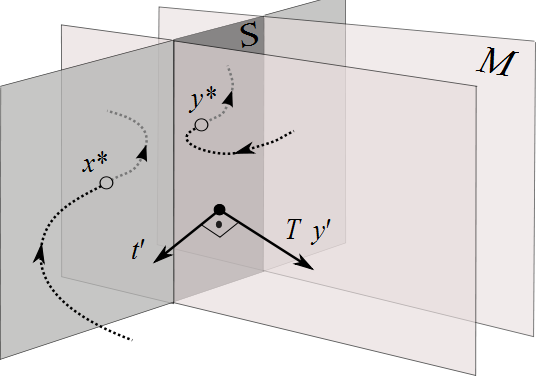
\includegraphics[width=0.90\textwidth]{inflectHype3D.png}
 \end{center}
 \caption{\label{fig:inflectHype3D}
Two hyperplanes are associated with  any given {\template} \slicep; the
slice $\pSRed$, and the hyperplane of points $\sspSing$, points for which
the curvature of the distance function \refeq{minDistance} changes sign.
For rotation angles beyond this hyperplane the group orbit
$\LieEl\,\ssp$ has left the {\template} neighborhood. For $\SOn{2}$ this
hyperplane is normal to the quadratic Casimir-weighted vector
$\Lg^2\slicep$. The intersection of the two hyperplanes is the {\em
\sset} $\sspRSing \in S$, within which the group tangent
$\groupTan(\sspRSing)$ points into the slice and is thus normal to
$\sliceTan{}$.
 }%
 \end{figure}

\item[2011-01-25 ES] Revert! Revert! That's even worse. Sorry, what I meant is that the
figure is not clearly labeled so that one could understand that $S$ is the
vertical axis. Also that it perhaps should not be aligned with the coordinate
axis but be another 1-D line? Does it ought to lie along the axis? I don't
think one can plot higher dimensional hyperplanes intersecting in any
meaningful way, no matter how European one is (even the French can't do that!).


\item[2011-01-25 PC] \Slice s, \sset s and ridges all include the
fixed-point subspace, which is \cLe\ case is the $z$ axis, that's why I
think it ought to lie along the axis. I've modified the caption of the
original figure to explain that $S$ is not a `line', will commit that
tomorrow when I get back to my work computer.

\item[2012-02-25 PC] all exercises moved to ChaosBook, exerFlow.tex
removed.

\item[2012-02-25 PC] all flotsam moved all to atlas, flotsamFrCv11.tex
removed.


\end{description}
